%%%%%%%%%%%%%%%%%%%%%%%%%%%%%%%%%%%%%%%%%%%%%%%%%%%%%%%%%%%%%%%%%%%%%%%%%%%%%%%%%%%%
% Do not alter this block (unless you're familiar with LaTeX
\documentclass{article}
\usepackage[margin=1in]{geometry} 
\usepackage{amsmath,amsthm,amssymb,amsfonts, fancyhdr, color, comment, graphicx, environ}
\usepackage{xcolor}
\usepackage{mdframed}
\usepackage[shortlabels]{enumitem}
\usepackage{indentfirst}
\usepackage{hyperref}
\usepackage{algorithm2e}
\usepackage{graphicx}
\usepackage{wrapfig}
\usepackage{hyperref}
\usepackage{listings}
\lstset{ 
  language=R,                     % the language of the code
  basicstyle=\normalsize\ttfamily, % the size of the fonts that are used for the code
  numbers=left,                   % where to put the line-numbers
  numberstyle=\normalsize\color{gray},  % the style that is used for the line-numbers
  stepnumber=1,                   % the step between two line-numbers. If it is 1, each line
                                  % will be numbered
  numbersep=5pt,                  % how far the line-numbers are from the code
  backgroundcolor=\color{white},  % choose the background color. You must add \usepackage{color}
  showspaces=false,               % show spaces adding particular underscores
  showstringspaces=false,         % underline spaces within strings
  showtabs=false,                 % show tabs within strings adding particular underscores
  frame=single,                   % adds a frame around the code
  rulecolor=\color{black},        % if not set, the frame-color may be changed on line-breaks within not-black text (e.g. commens (green here))
  tabsize=2,                      % sets default tabsize to 2 spaces
  captionpos=b,                   % sets the caption-position to bottom
  breaklines=true,                % sets automatic line breaking
  breakatwhitespace=false,        % sets if automatic breaks should only happen at whitespace
  keywordstyle=\color{black},      % keyword style
  commentstyle=\color{gray},   % comment style
  stringstyle=\color{teal}      % string literal style
} 
\hypersetup{
    colorlinks=true,
    linkcolor=blue,
    filecolor=magenta,      
    urlcolor=blue,
}


\pagestyle{fancy}


\newenvironment{problem}[2][Problem]
    { \begin{mdframed}[backgroundcolor=gray!20] \textbf{#1 #2} \\}
    {  \end{mdframed}}

% Define solution environment
\newenvironment{solution}
    {\textit{Solution:}}
    {}

\renewcommand{\qed}{\quad\qedsymbol}

% prevent line break in inline mode
\binoppenalty=\maxdimen
\relpenalty=\maxdimen

%%%%%%%%%%%%%%%%%%%%%%%%%%%%%%%%%%%%%%%%%%%%%
%Fill in the appropriate information below
\lhead{Pengju Zhang \href{run:./src/about/index.html}{ (About Me)}}
\rhead{CSC-424} 
\chead{\textbf{Assignment 1}}
%%%%%%%%%%%%%%%%%%%%%%%%%%%%%%%%%%%%%%%%%%%%%

\begin{document}
%problem 1
\begin{problem}{1}
\textbf{[20 pts]}
Looking beyond the surface. While we will be spending a great deal of time learning more sophisticated model building techniques, often the immediate “parameter of interest” that seems to appear in a dataset is not the most interesting/impactful one, nor are the original variables necessarily in a form that is best for modeling the data. This problem asks you to look below the surface to find a story in the data that is more interesting than the obvious one.
\newline
The Olympics data set concerns the performance of various countries in the 2012 London Summer Olympics. For each country, the data contains separate medal counts, number of athletes by gender, national population figures, and national gross domestic product (GDP). The obvious surface message in the data is that larger countries/teams with higher GDP generally win more medals. It is your job to distill an interesting story or insight in this data, but it should be something other than the obvious positive relationship between raw or aggregate medal counts and population/GDP.
\newline
It will take some investigation to find a suitable message, and you should look at several relationships, and consider transforming/creating some new variables based on the original variables before settling on one. There are several opportunities for interesting analyses in this data and you do not need to investigate all of them. Think about whether there is an important trend or lesson that you would like the public to understand? Below are some things to consider. You do not have to investigate all of these. They are provided to help you think about the data.
\begin{enumerate}
	\item Do any surprises emerge? Often, the most interesting results are surprising ones because they tell us things we didn’t expect.
	\item Are there any transformations or ways of combining variables that can reveal more subtle patterns than simply overall population/GDP? What about per-capita or per-participant measures? Is there any relationship between participation of certain demographics and the country’s performance?
	\item Imagine you are an Olympic coach for a small country, what does performance mean if your country has limited resources? The GDP/team size vs. medal count relationships merely say, “grow your economy and increase your team size (larger budget) to win more medals.” Is there a way of marginally improving the performance of the athletes you have (how would you measure that)? Even if the resulting model does not have a high R2, it can still be practically significant.
	\item Are there ways to evaluate a country's "performance" beyond medal counts? Are there any relationships that have nothing do to with medal performance that are interesting or impactful?
	\item Sometimes the most interesting results are not in the nature of the model but in the nature of the outliers. These outliers can suggest directions for future study.
\end{enumerate}
Sometimes the most interesting results are not in the nature of the model but in the nature of the outliers. These outliers can suggest directions for future study.
\newline
You may try different multiple-regressions and plots and can compare these results to automatic variable selection methods, but your writeup should only include your best, most interesting analysis. Be thorough but concise in your write-up and be sure to include the graph(s) and analyses you are using to see the relationships and clearly indicate the intended message of your analysis. There are many possible relationships to consider but you will be graded on the clarity and the thoroughness of your graphs and written analysis. You should be able to fill at least a page.
\end{problem}
\newpage
\begin{solution}
\href{run:./src/RCode/p1.r}{ (Problem 1 Source Code)}
\newline
In my opinion, although different medals mean different honors for individuals, but total quantity of medals is more accurate factor to compare each country, so I add a total medals as one variable. And another indicator is GDP per capita, I leave both of them in my data pre-process step.
	\begin{lstlisting}
	data = read.csv("olympics.csv")
	str(data)
	data$GDP.per.capita <- (data$X2011.GDP/data$X2010.population)
	data$Total.medals <- (data$Gold.medals+data$Silver.medals+data$Bronze.medals)
	\end{lstlisting}
One fast way to quick look at relation among all variables is through correlation matrix plot.
	\begin{lstlisting}
	library(psych)
	# country code and name is not necessary
	pairs.panels(data[,-c(1,2)])
	\end{lstlisting}
	\begin{figure}[h]
		\centering
		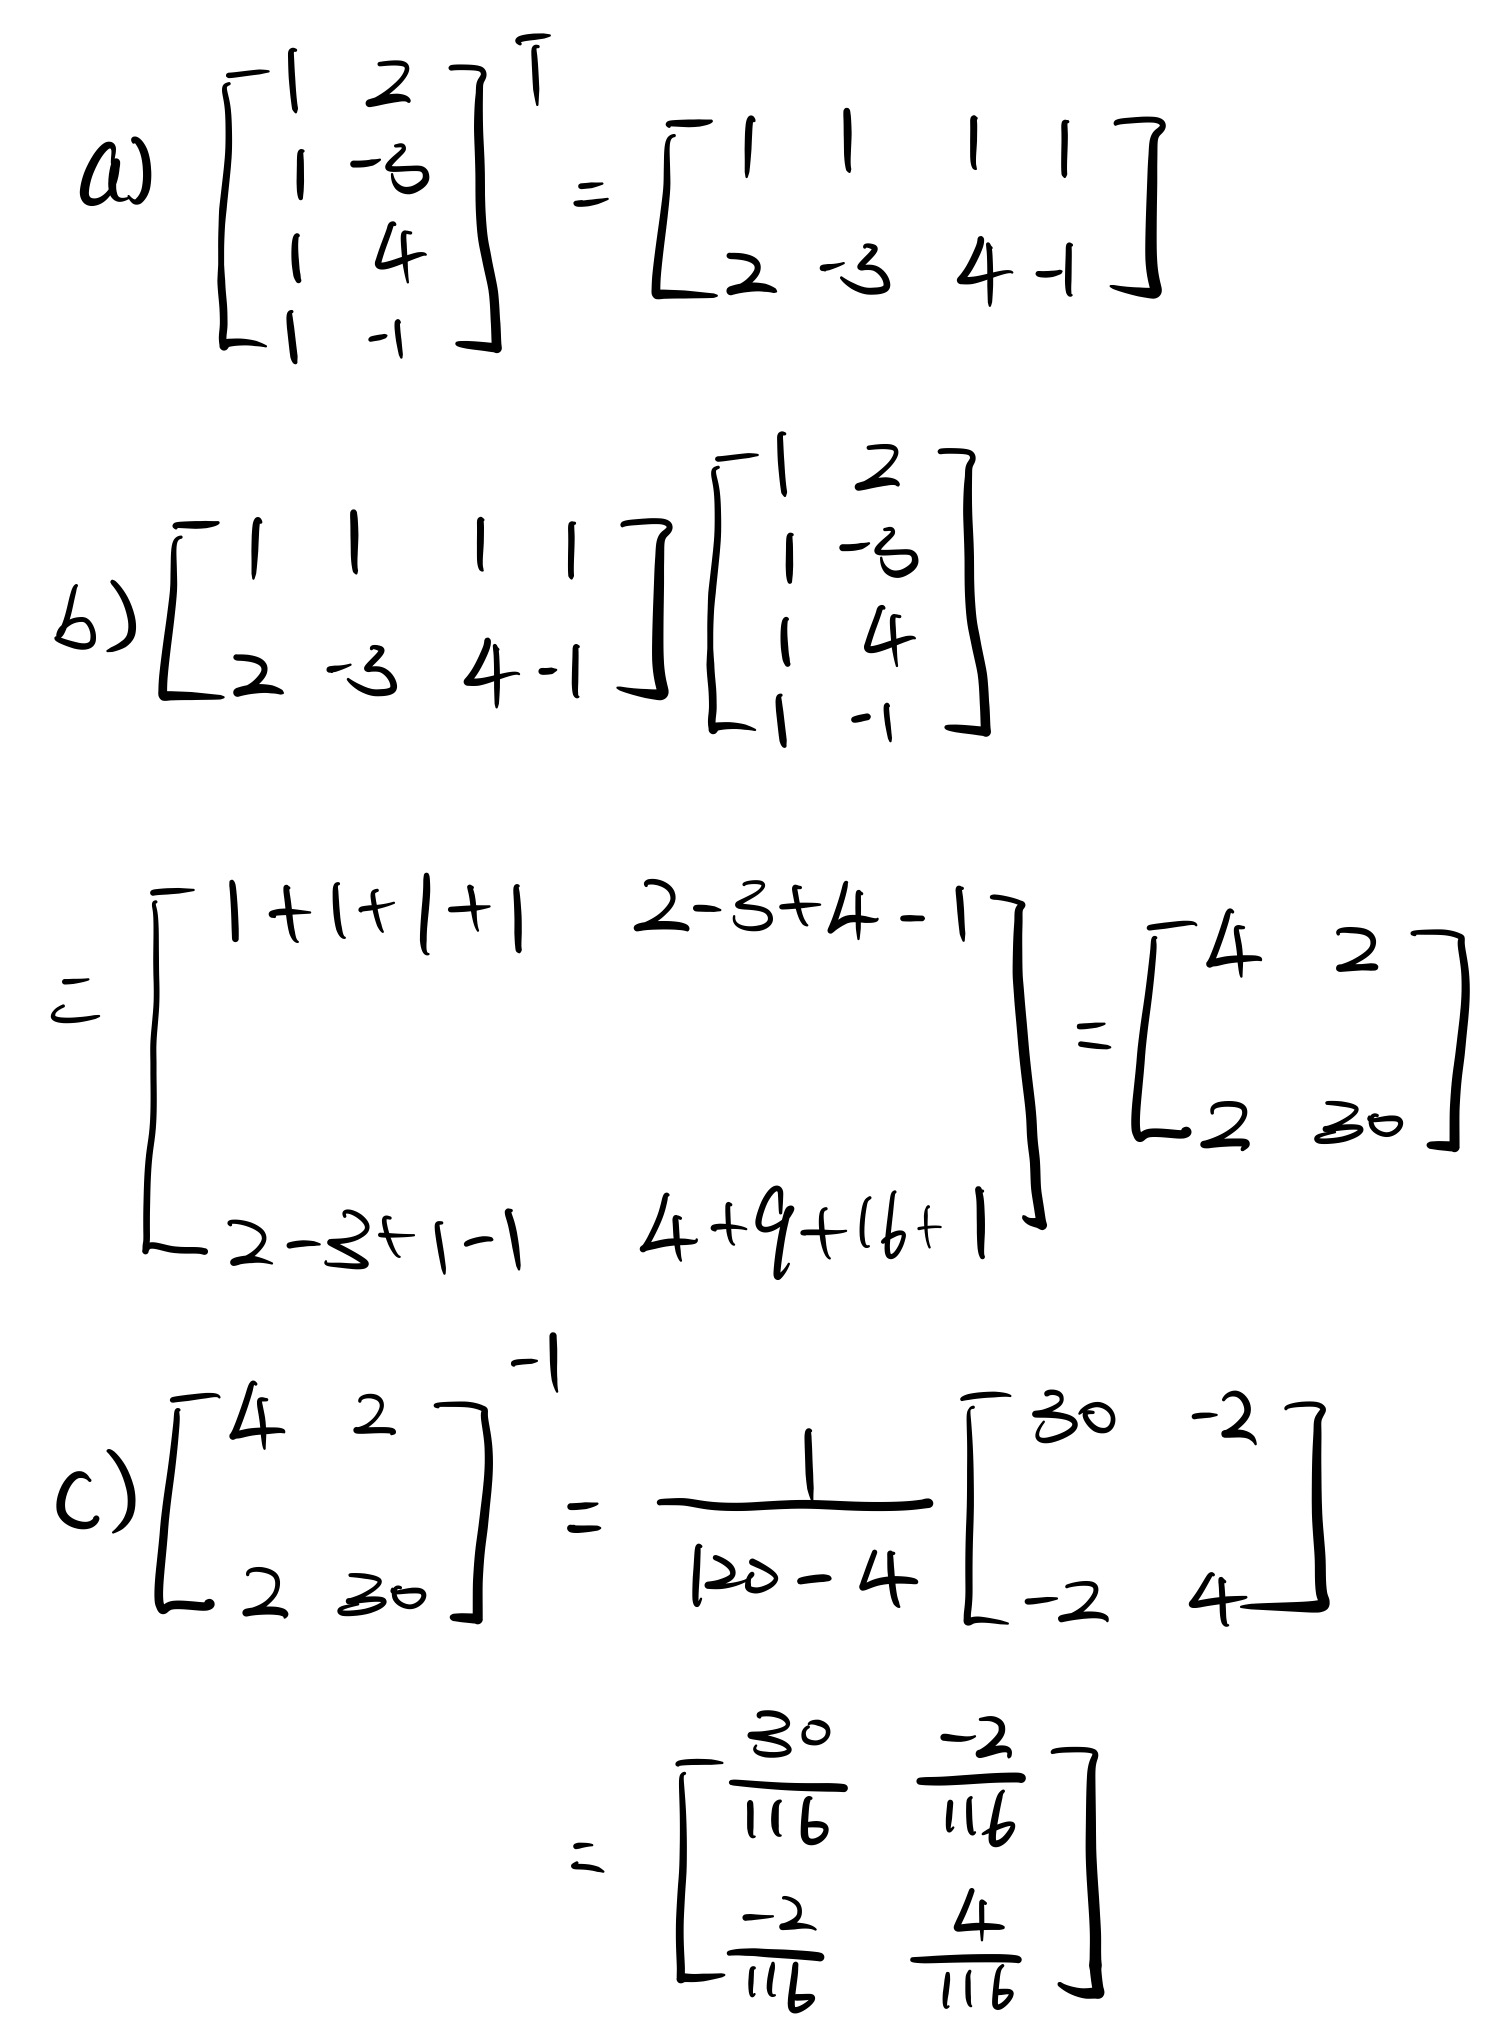
\includegraphics[width=0.5\textwidth]{figure1_Rplot.jpeg}
		\caption{2012 London Olympics Dataset Correlation Matrix}
	\end{figure}
If I just look at the last column what I find more surprising are two things, one is that the total number of medals has a strong positive correlation with GDP more than GDP per capita. Secondly, the correlation is slightly stronger for the total number of women than men.
\newline
The first point actually makes sense, after all, more money means more athletes can be trained, so more medals are won. The second point can be understood if you look at the data carefully, because most countries have more female participants than male.
\newpage
In this case I may choose the male/female ratio to normalize difference number between then, and ratio between GDP and total participants might be an interesting transformation.
	\begin{lstlisting}
	# add ratio between GDP and total participants
	data$GDP.per.participants <- (data$X2011.GDP/(data$Male.count+data$Female.count))
	pairs.panels(data[,-c(1,2)])
	\end{lstlisting}
	\begin{figure}[h]
		\centering
		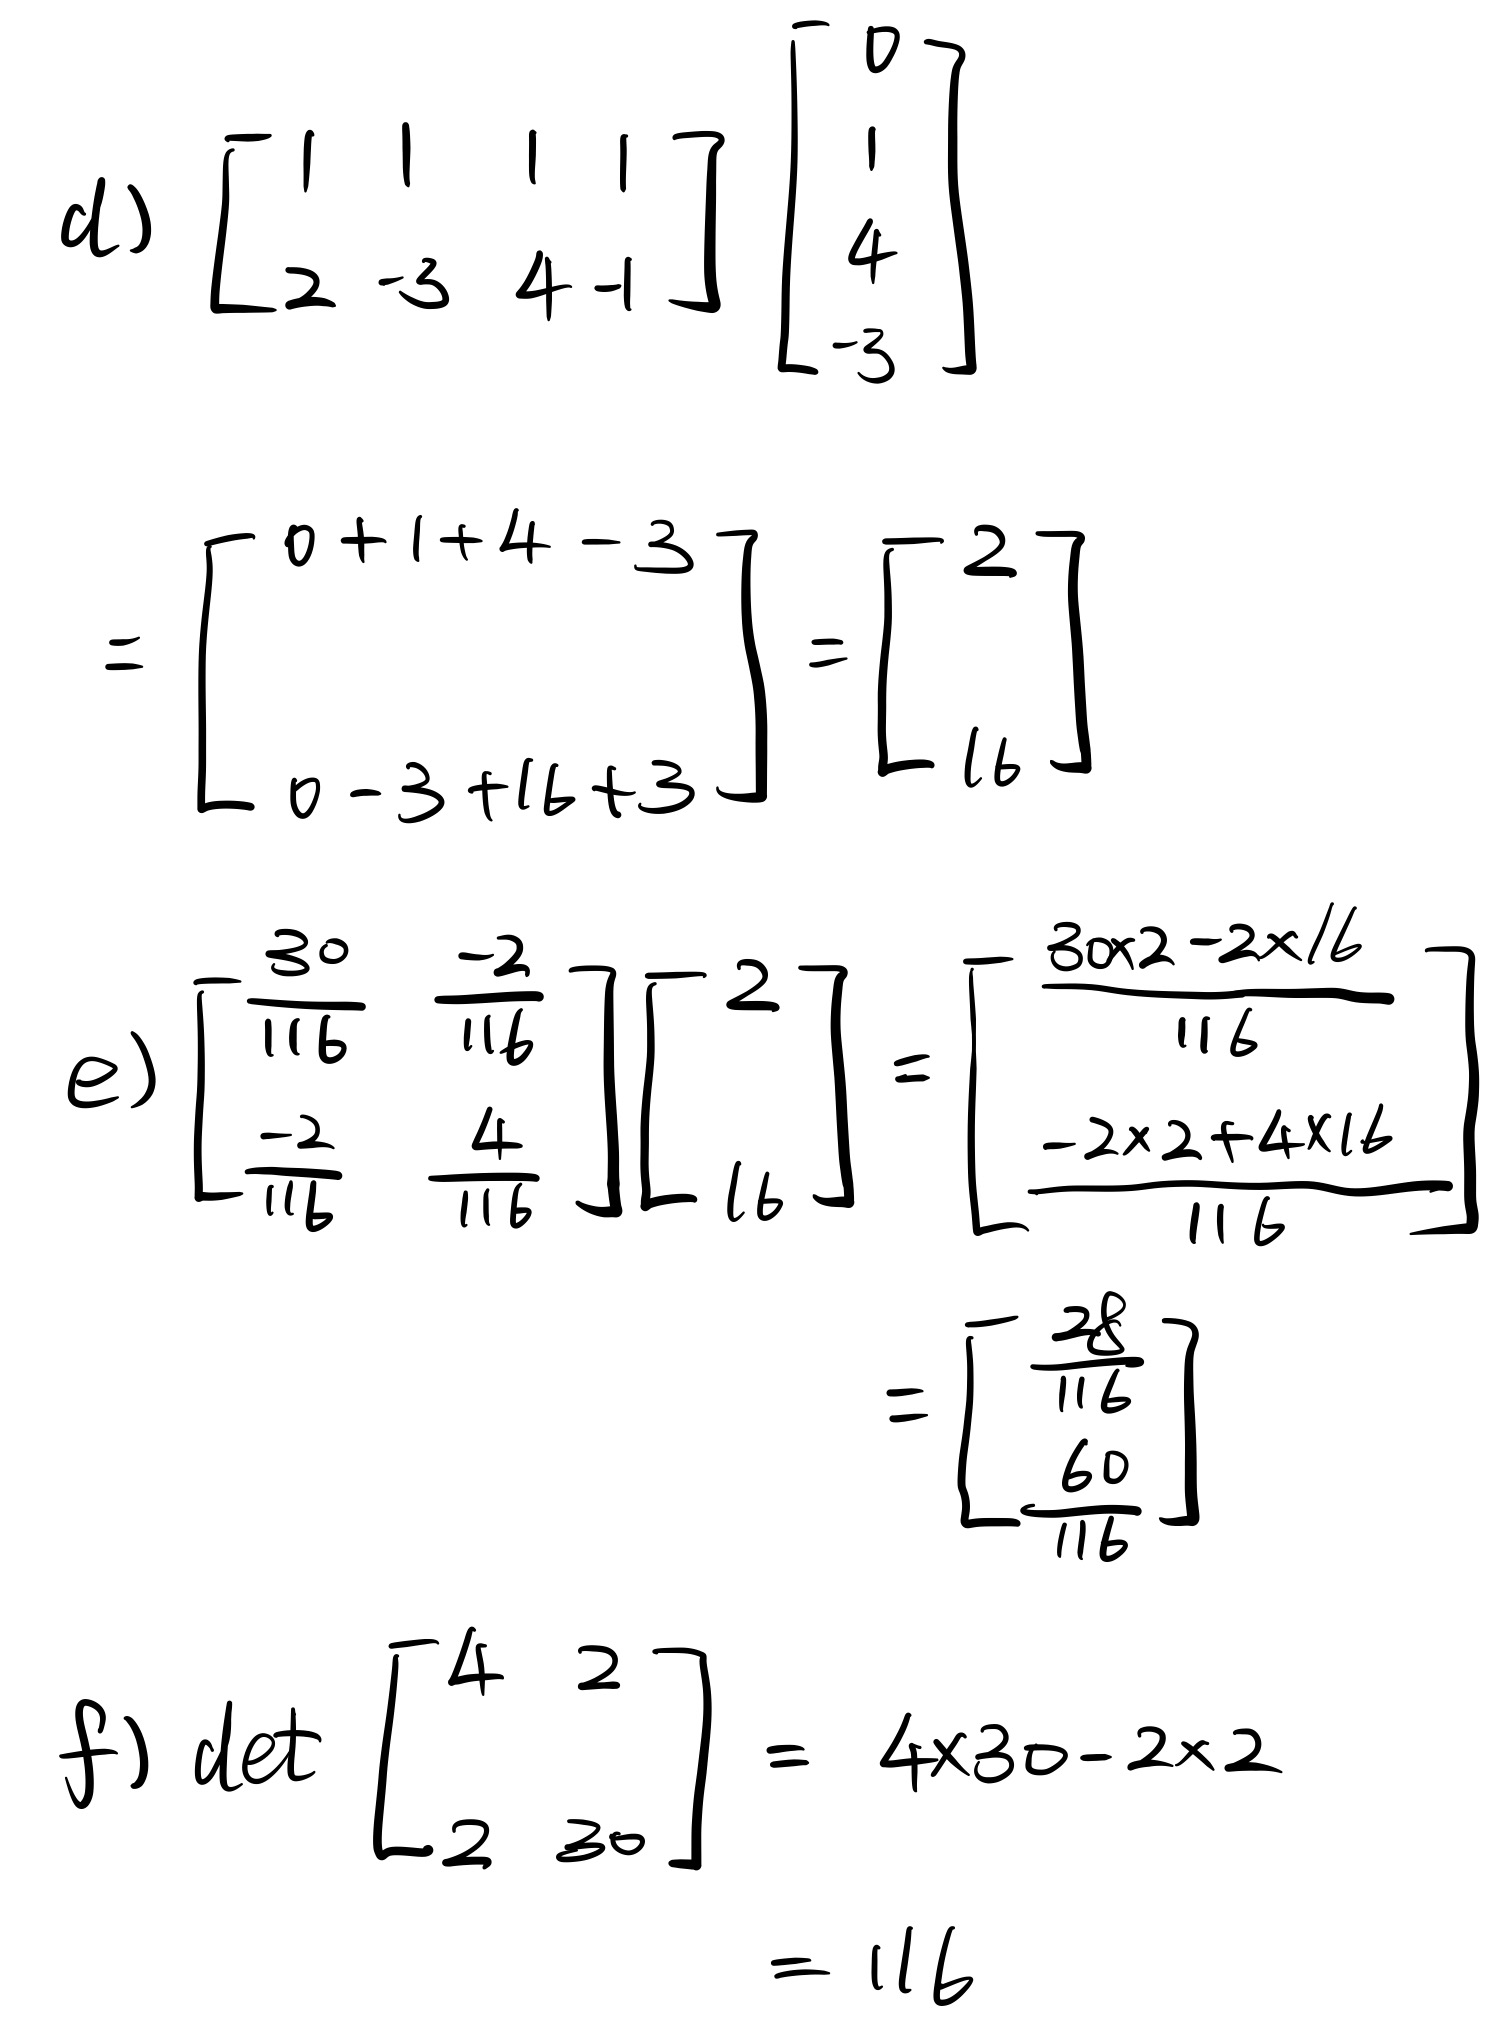
\includegraphics[width=0.5\textwidth]{figure2_Rplot.jpeg}
		\caption{2012 London Olympics Dataset Correlation Matrix}
	\end{figure}
Matrix figure shows GDP per participants is not quite good factor to add since it has low correlation to all others. If I treat total medals as performance, depends on correlation there are three factors that I would like to know more about.
	\begin{lstlisting}
	attach(data)
	# 3 highly correlated factors Female.count,  Male.count and X2011.GDP
	fit = lm(Total.medals ~ Female.count + Male.count + X2011.GDP)
	summary(fit)
	plot(fit)
	library(car)
	vif(fit)
	\end{lstlisting}
\newpage
	\begin{figure}[h]
		\centering
		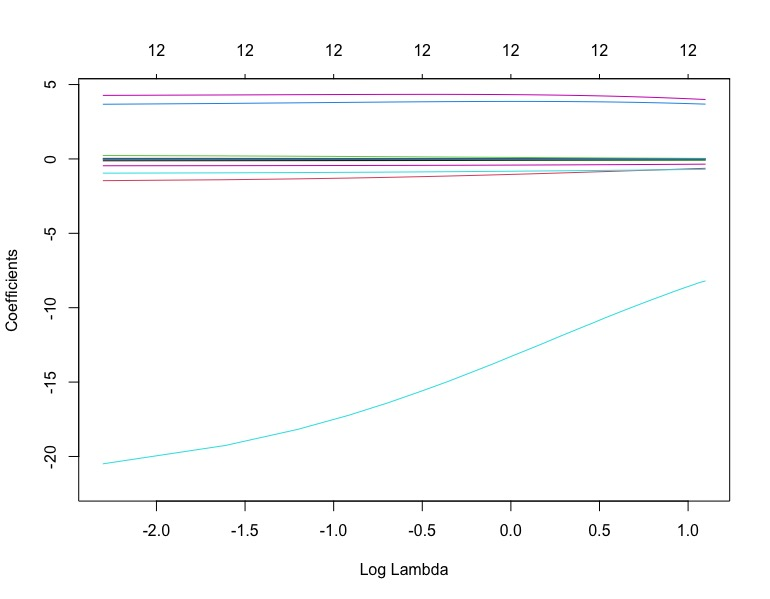
\includegraphics[width=0.5\textwidth]{figure3_Rplot.jpeg}
		\caption{Residuals vs Linear Fitted Model}
		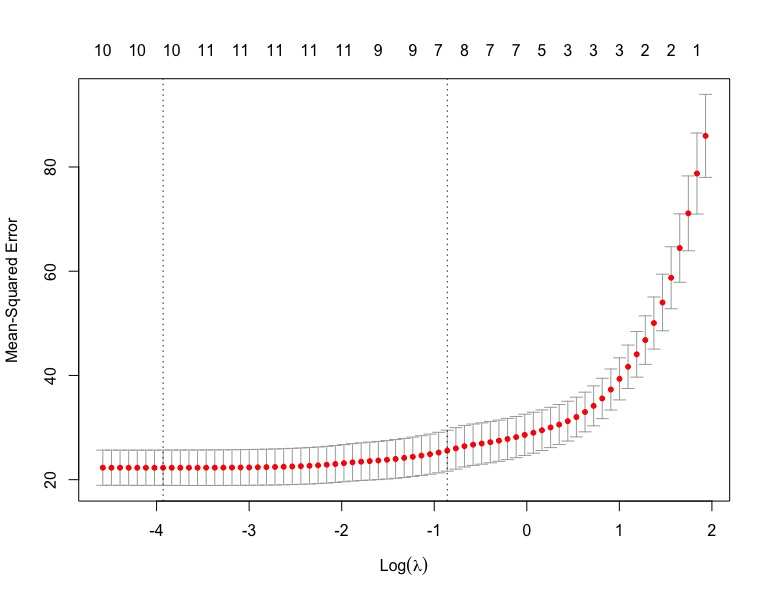
\includegraphics[width=0.5\textwidth]{figure4_Rplot.jpeg}
		\caption{Normal Q-Q of Linear Fitted Model}
	\end{figure}
From this model it can be seen that there are quite a few outliers, VIF of 22.098889 for female count and 18.630996 for male count indicate the high multicollinearity. This might be cause by lack of dataset, because there is no way to determine the relation between gender and medals. 
\newpage
To improve our model, I want to combine female and male together as total participants. 
	\begin{lstlisting}
	data$Total.participants <-(data$Male.count+data$Female.count)
	fit2 = lm(Total.medals ~ Total.participants + X2011.GDP)
	\end{lstlisting}
	\begin{lstlisting}
	pairs.panels(data[,-c(1,2)])
	\end{lstlisting}
	\begin{figure}[h]
		\centering
		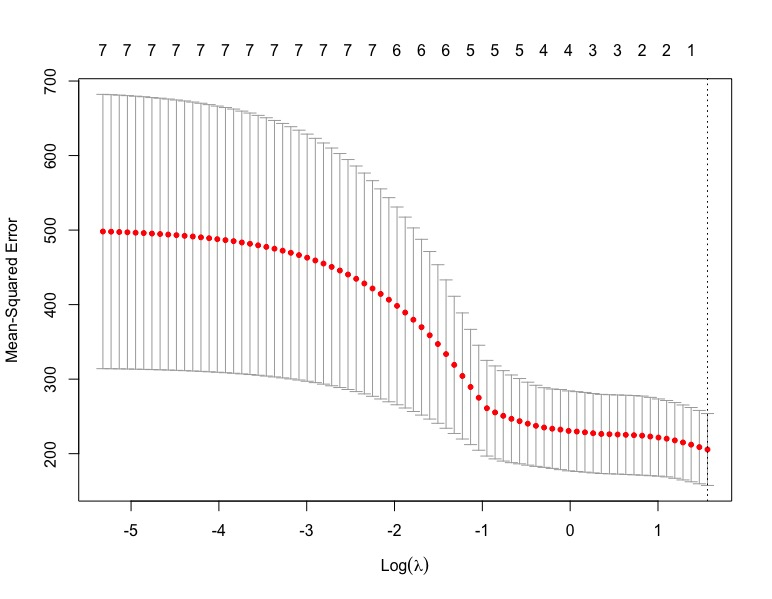
\includegraphics[width=0.5\textwidth]{figure5_Rplot.jpeg}
		\caption{2012 London Olympics Dataset Correlation Matrix}
	\end{figure}
	\begin{lstlisting}
	summary(fit2)
	#Coefficients:
         #Estimate Std. Error t value Pr(>|t|)    
	#(Intercept)        -1.663e+00  3.881e+00  -0.428   0.6737    
	#Total.participants  1.147e-01  2.069e-02   5.541 3.59e-05 
	#X2011.GDP           2.985e-12  1.083e-12   2.757   0.0135  
	#---
	#Residual standard error: 12.02 on 17 degrees of freedom
	#Multiple R-squared:  0.8806,	Adjusted R-squared:  0.8665 
	#F-statistic: 62.69 on 2 and 17 DF,  p-value: 1.428e-08
	\end{lstlisting}
\newpage
	\begin{lstlisting}
	plot(fit2)
	\end{lstlisting}
	\begin{figure}[h]
		\centering
		\includegraphics[width=0.5\textwidth]{figure6_Rplot.jpeg}
		\caption{Normal Q-Q of Linear Fitted Model}
	\end{figure}
	\begin{lstlisting}
	vif(fit2)
	# Total.participants          X2011.GDP 
          # 2.078394           2.078394 
	\end{lstlisting}
Correlation between new variable, Total.participants, and Total.medals has fairy strong positive index of 0.91 (Figure 5) . Once we transform the data into only 3 variables, we can see a significant change in outlier, only two left, China and Russia (Figure 6). VIF of 2.078394 for total participants and 2.078394 for GDP indicate the low multicollinearity.
\newline
To further improve my model, I want to exclusive these two outliers from my dataset.
	\begin{lstlisting}
	finalModel = data[-c(2, 9), -c(1,2)]
	attach(finalModel)
	fit3 = lm(Total.medals ~ Total.participants + X2011.GDP)
	summary(fit3)
	#Coefficients:
	#Estimate Std. Error t value Pr(>|t|)    
	#(Intercept)        -8.468e-01  1.994e+00  -0.425    0.677    
	#Total.participants  8.599e-02  1.188e-02   7.240 2.88e-06 
	#X2011.GDP           3.517e-12  6.078e-13   5.786 3.59e-05 
	#---
	#Residual standard error: 6.142 on 15 degrees of freedom
	#Multiple R-squared:  0.957,	Adjusted R-squared:  0.9512 
	#F-statistic: 166.7 on 2 and 15 DF,  p-value: 5.685e-11
	\end{lstlisting}
	\begin{lstlisting}
	vif(fit3)
	#Total.participants          X2011.GDP 
	#2.248135           2.248135 
	\end{lstlisting}
Adjusted $R^2$ increased from 	0.8665 to 0.9512 , and VIF still in good range, I would like to introduce my final model.
\begin{equation}
	Total Medals = -0.08468 + Total.participants\times 8.599\times 10^{-2} + X2011.GDP\times 3.517\times 10^{-12}
\end{equation}
\newline
From the model, there are only two variables have a positive impact on total medals. In terms of economic volume, it is difficult to surpass large countries, but there are still opportunities in retrospect. China is a good example of been good at olympics in 1950s, they chose table tennis as their entry game, which had two advantages, firstly, it required very little space, which could significantly reduce the capital investment, and secondly, table tennis was a niche sport in that period, which could be easily achieved in a very short period of time. If I am an Olympic coach for a small country, these two points will be my primary consideration.
\newline
In addition, Olympic Games is entirely a competition between the size of countries, small countries have lost at the starting line. But I think as a competitive sport, some soft conditions such as unfair treatment by the host country and drug abuse should be taken into account as performance.
\end{solution}

\newpage
%problem 2
\begin{problem}{2}
\textbf{[25 pts]}
The Housing dataset housing.csv contains a modified version of a dataset of housing values. One parameter has been dropped from the original dataset due to its very slight contribution to the parameter of interest and its biased and mathematically flawed nature.
\begin{enumerate}
	\item\textbf{(5 pts)} Fit an initial linear regression model of MEDV based on all the other variables and report $R^2$, Adjusted $R^2$, the utility of the model (F-Test), the estimated coefficients, their standard errors, and statistical significance. Interpret your results. Treat the RAD ordinal variable as numeric.
	\item\textbf{(5 pts)} Plot the dataset in a scatterplot matrix and also the correlation with a corrplot. Interpret the result. Are there variables whose correlation with MEDV are weak? Are their variables whose relationship to MEDV are non-linear, or for which a log transform should be applied (look for a lot of samples on the axis with relatively few at high values)? Look for at least two transformations to apply that can increase the $R^2$ value of the regression. Transform the variables, rerun the regression, and compare the results to the initial regression.
	\item\textbf{(5 pts)} Perform a feature selection on the transformed data by using the stepwise selection method of the regression analysis. Which variables are dropped in the stepwise selection model and how is the adjusted $R^2$ affected? Evaluate the result in comparison to the full model.
	\item\textbf{(5 pts)} Perform an all-subsets analysis with “regsubsets” (set the “nvmax” parameter high enough that the search will include the regression with all the variables). Write out the model as an equation, plot and interpret the results (using the adjusted $R^2$ value on the vertical axis). What variables are dropped in the “best” model and how does it compare to the stepwise model? Leave the parameter “nbest” at its default of 1 to reduce the complexity of the graph.
	\item\textbf{(5 pts)} Suppose you were trying to find parsimonious model (i.e. as few features as possible) to make the result easier to explain and use practically. Investigate the graph of the regsubsets result and determine if there is a model that reduces the number of variables significantly without significantly reducing adjusted $R^2$ (more than a percent or two). Explain your choice, and discuss which variables are included in the model? Compute that model with lm and interpret and compare the model practically with the stepwise model in terms of the effect of each variable on median house price.
\end{enumerate}
\end{problem}
\newpage
\begin{solution}
\href{run:./src/RCode/p2.r}{ (Problem 2 Source Code)}
	\begin{enumerate}
		\item\mbox{}
		\begin{lstlisting}
	housingData = read.csv("housing.csv")
	attach(housingData)
	fit = lm(MEDV ~ ., data=housingData)
		\end{lstlisting}
		\begin{lstlisting}
	summary(fit)
#Residuals:
#     Min       1Q   Median       3Q      Max 
#-15.1304  -2.7673  -0.5814   1.9414  26.2526 
#Coefficients:
#              Estimate Std. Error t value Pr(>|t|)    
#(Intercept)  41.617270   4.936039   8.431 3.79e-16 
#CRIM         -0.121389   0.033000  -3.678 0.000261 
#ZN            0.046963   0.013879   3.384 0.000772 
#INDUS         0.013468   0.062145   0.217 0.828520    
#CHAS          2.839993   0.870007   3.264 0.001173  
#NOX         -18.758022   3.851355  -4.870 1.50e-06 
#RM            3.658119   0.420246   8.705  < 2e-16 
#AGE           0.003611   0.013329   0.271 0.786595    
#DIS          -1.490754   0.201623  -7.394 6.17e-13 
#RAD           0.289405   0.066908   4.325 1.84e-05 
#TAX          -0.012682   0.003801  -3.337 0.000912 
#PTRATIO      -0.937533   0.132206  -7.091 4.63e-12 
#LSTAT        -0.552019   0.050659 -10.897  < 2e-16 
#---
#Residual standard error: 4.798 on 493 degrees of freedom
#Multiple R-squared:  0.7343,	Adjusted R-squared:  0.7278 
#F-statistic: 113.5 on 12 and 493 DF,  p-value: < 2.2e-16
		\end{lstlisting}
The residuals of model is quite symmetric but not perfect, the median is close to 0, first and third quartile are close in magnitude, but min and max have hug difference.
	\begin{figure}[h]
		\centering
		\includegraphics[width=0.5\textwidth]{figure7_Rplot.jpeg}
		\caption{Normal Q-Q of Linear Fitted Model}
	\end{figure}
\newpage
In this case, $R^2 = 0.7343$ and adjusted $R^2 = 0.7278$ indicate a moderate positive correlation, and it gives a measurement of 73 percent of the variance in the response variable can be explained by the linear regression. Lastly, the p-value of F-test is much smaller than 0.05 indicate the whole model is statistically significant.
	\item\mbox{}
	\begin{lstlisting}
	# correlation scatterplot matrix
	library(psych)
	pairs.panels(housingData)
	\end{lstlisting}
	\begin{figure}[h]
		\centering
		\includegraphics[width=0.5\textwidth]{figure8_Rplot.jpeg}
	\caption{Housing Data Correlation Scatterplot Matrix}
	\end{figure}
	\begin{lstlisting}
	# correlation scatterplot with a corrplot
	library(corrplot)
	cor.hbat = cor(housingData)
	corrplot(cor.hbat)
	\end{lstlisting}
		\begin{figure}[h]
		\centering
		\includegraphics[width=0.5\textwidth]{figure9_Rplot.jpeg}
		\caption{Housing Data Correlation Scatterplot Matrix}
	\end{figure}
\newpage
Both CHAS and DIS has very weak correlation with MEDV. Since CHAS is categorical variable, it is reasonable to have weak correlation with all other variables, DIS has a right skewed distribution in figure 8, this might be considered to normalized and re-run in our linear regression. Same reason as DIS, there are two other variables need logistic transformation which are NOX and LSTAT.
	\begin{lstlisting}
	logDis = log(housingData$DIS)
	housingData$DIS = logDis
	attach(housingData)
	fit = lm(MEDV ~ ., data=housingData)
	summary(fit)
# output
# Multiple R-squared:  0.7556,	Adjusted R-squared:  0.7497 
	\end{lstlisting}
Log transformation of DIS increased $R^2$ from 0.7343 to 0.7556.
	\begin{lstlisting}
	logNOX = log(housingData$NOX)
	housingData$NOX = logNOX
	attach(housingData)
	fit = lm(MEDV ~ ., data=housingData)
	summary(fit)
# output
# Multiple R-squared:  0.7541,	Adjusted R-squared:  0.7481 
	\end{lstlisting}
Log transformation of NOX has negative impact, so I keep NOX same as original data.
	\begin{lstlisting}
	logLSTAT = log(housingData$LSTAT) 
	housingData$LSTAT = logLSTAT
	attach(housingData)
	fit = lm(MEDV ~ ., data=housingData)
	summary(fit)
# output
# Multiple R-squared:  0.8005,	Adjusted R-squared:  0.7956 
	\end{lstlisting}
Log transformation of LSTAT increased $R^2$ from 0.7556 to 0.8005. Consequently, I choose log transformation for DIS and LSTAT.
	\item\mbox{}
	\begin{lstlisting}
# stepwise selection
	null = lm(MEDV ~ 1, data=housingData)
	full = lm(MEDV ~ ., data=housingData)
# forward
	housingForward = step(null, scope = list(lower=null, upper=full), direction="forward", trace=F)
	summary(housingForward)
# output
# Multiple R-squared:  0.7992,	Adjusted R-squared:  0.7955
	\end{lstlisting}
Forward selection remove 2 variables, ZN and INDUS. Adjusted do not have any change compare to the previous model of 0.8005.
\newpage
	\begin{lstlisting}
#backward
	housingBackward = step(full, scope=list(lower=null, upper=full), direction="backward", trace=F)
	summary(housingBackward)
# output
# Multiple R-squared:  0.7992,	Adjusted R-squared:  0.7955
	\end{lstlisting}
Backward selection remove ZN and INDUS as well, so $R^2$ keep same as forward selection.
	\item\mbox{}
	\begin{lstlisting}
	library(leaps)
	housingSubsets = regsubsets(MEDV ~ ., data=housingData, nvmax=13, nbest=1)
	reg.summary = summary(housingSubsets)
	plot(reg.summary$rsq, xlab="Number of Variables", ylab="RSquare", type="l")
	\end{lstlisting}
	\begin{figure}[h]
		\centering
		\includegraphics[width=0.5\textwidth]{figure10_Rplot.jpeg}
		\caption{Changes in $R^2$ Respect to Number of Variables}
	\end{figure}
As far as we can see, when we include more than 8 variables, the $R^2$ reach to its maximum around 0.8.
\newpage
	\begin{lstlisting}
	plot(housingSubsets, scale="adjr2")
	\end{lstlisting}
	\begin{figure}[h]
		\centering
		\includegraphics[width=0.8\textwidth]{figure11_Rplot.jpeg}
		\caption{Best Subsets Selection with Adjusted $R^2$}
	\end{figure}	
The best model in this case is 0.8 of adjusted $R^2$ without ZN, INDUS and AGE.
	\begin{lstlisting}
	bestR2Fit = lm(MEDV ~ .-INDUS-AGE-ZN, data=housingData)
	summary(bestR2Fit)
# Multiple R-squared:  0.7992,	Adjusted R-squared:  0.7955 
	\end{lstlisting}
Compare to the stepwise selection, there is no change on $R^2$, but we have removed one  negligible variable, Age.
\newpage
	\item\mbox{}
0.79 adjusted $R^2$ would be the my best choice since CHAS has least impact on the whole model.
	\begin{lstlisting}
	library(lm.beta)
	stdCoef = coef(lm.beta(housingForward))    
	barplot(rev(sort(stdCoef)))  
	\end{lstlisting}
	\begin{figure}[h]
		\centering
		\includegraphics[width=0.8\textwidth]{figure12_Rplot.jpeg}
		\caption{Coefficients of Each Variable's Influence}
	\end{figure}		
	\begin{lstlisting}
	finalModel = lm(MEDV ~ .-INDUS-AGE-ZN-CHAS, data=housingData)
	summary(finalModel)
# Multiple R-squared:  0.7954,	Adjusted R-squared:  0.7921 
	\end{lstlisting}
	\begin{lstlisting}
	library(car)
	vif(finalModel)
#    CRIM      NOX       RM      DIS      RAD      TAX  PTRATIO    LSTAT 
1.754071 4.289744 1.923598 3.517214 6.813674 6.980374 1.555594 2.709693
	\end{lstlisting}
by removing CHAS we only have 0.0034 down on adjusted $R^2$ compare to best model, and VIFs are in the accepted range, as the result our final model would be
\begin{equation}
\begin{split}
	MEDV & = 67.449453 - 0.177755\times CRIM - 21.617400\times NOX \\ 
	& + 2.657238\times RM - 7.029076\times log(DIS) + 0.321142\times RAD \\
	& - 0.013970\times TAX - 0.894041\times PTRATIO - 9.066324\times log(LSTAT)
\end{split}
\end{equation}		
	\end{enumerate}
\end{solution}

\newpage
%problem 3
\begin{problem}{3}
\textbf{[20 pts]}
Perform, by hand, the following calculations from linear algebra. For the following matrices and vectors. Submit a clear and easy to read scan or photo. Particularly if you are using a cell phone, make sure that your page is well framed and is square with the camera. If your text is clipped off, blurred or taken at an angle that makes it difficult to read, it will not be graded.
\end{problem}
\begin{solution}
	\begin{figure}[h]
		\centering
		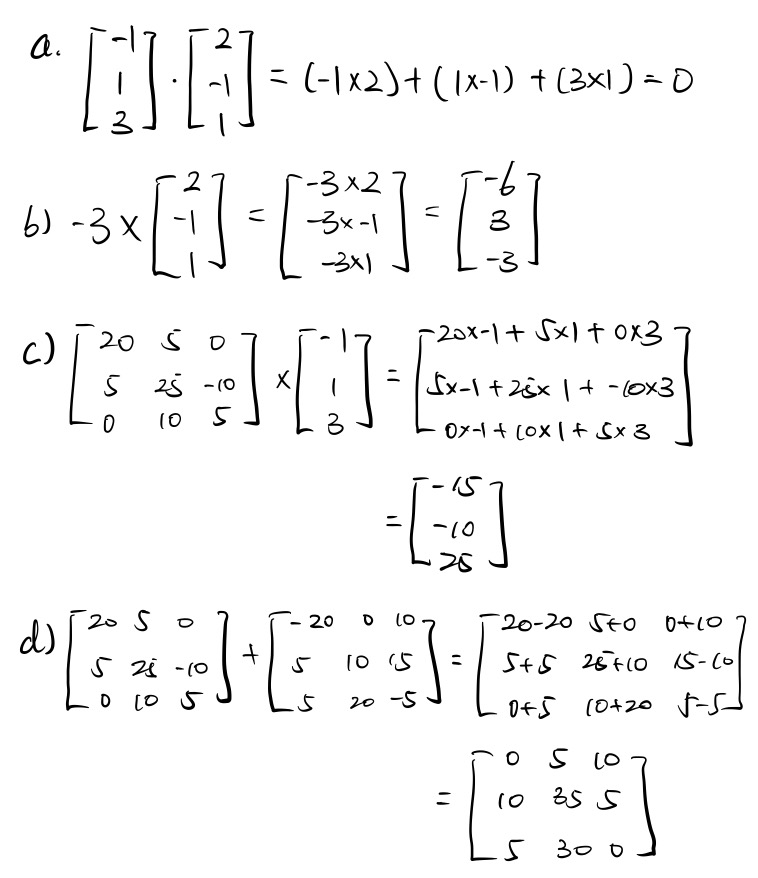
\includegraphics[width=0.8\textwidth]{p3_a.jpg}
	\end{figure}
\newpage
	\begin{figure}[h]
		\centering
		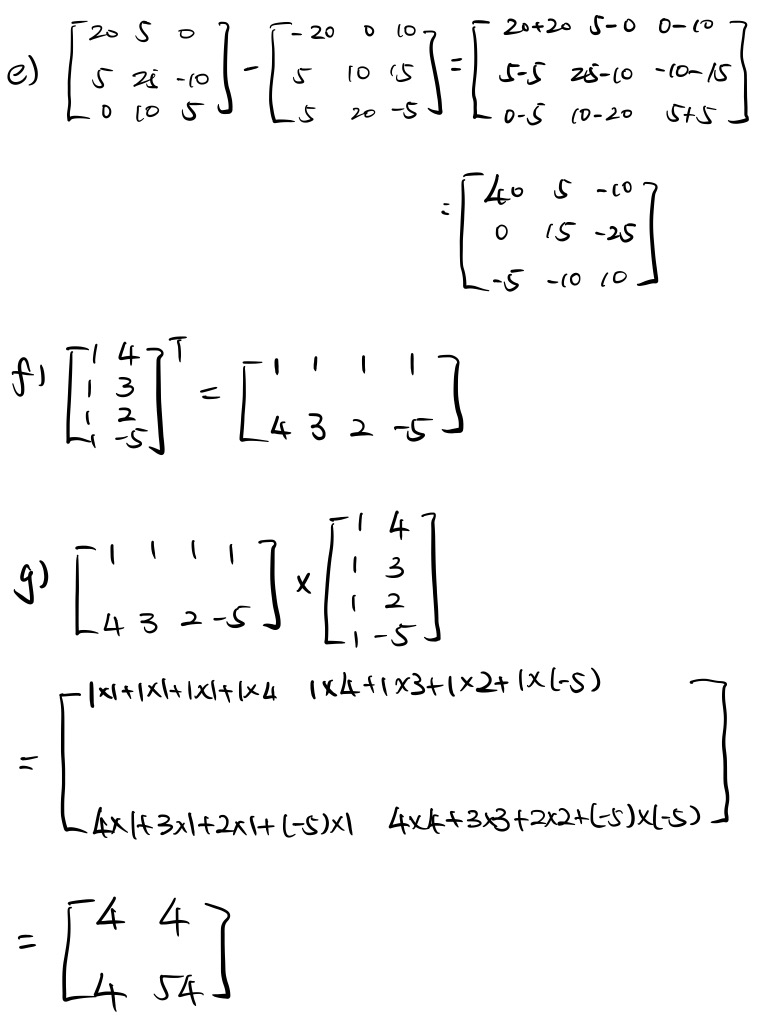
\includegraphics[width=0.8\textwidth]{p3_b.jpg}
	\end{figure}
\end{solution}

\newpage
%problem 4
\begin{problem}{4}
\textbf{[10 pts]}
In R, write a script to compute each of the parts in problem 4 to check your answers. Submit both the R code and the output. Make sure you correct any discrepancies in the answers, as they indicate that you have an issue either in your manual calculation or in your R code.
\end{problem}
\begin{solution}
\href{run:./src/RCode/p4.r}{ (Problem 4 Source Code)}
\begin{lstlisting}
# output
> p1
[1] 0
> p2
     [,1]
[1,]   -6
[2,]    3
[3,]   -3
> p3
     [,1]
[1,]  -15
[2,]  -10
[3,]   25
> p4
     [,1] [,2] [,3]
[1,]    0    5   10
[2,]   10   35    5
[3,]    5   30    0
> p5
     [,1] [,2] [,3]
[1,]   40    5  -10
[2,]    0   15  -25
[3,]   -5  -10   10
> p6
     [,1] [,2] [,3] [,4]
[1,]    1    1    1    1
[2,]    4    3    2   -5
> p7
     [,1] [,2]
[1,]    4    4
[2,]    4   54
\end{lstlisting}
\end{solution}
\end{document}